\newcommand{\lnext}{\ensuremath{\mathbf{X}}}
\newcommand{\lwnext}{\ensuremath{\mathbf{\bar{X}}}}
\newcommand{\luntil}{\ensuremath{\mathbf{U}}}
\newcommand{\lsince}{\ensuremath{\mathbf{S}}}
\newcommand{\lrelease}{\ensuremath{\mathbf{R}}}
\newcommand{\lwuntil}{\ensuremath{\mathbf{W}}}
\newcommand{\lglobally}{\ensuremath{\mathbf{G}}}
\newcommand{\lfuture}{\ensuremath{\mathbf{F}}}
\newcommand{\tnext}{\ensuremath{\mathbf{X}_{I}}}
\newcommand{\twnext}{\ensuremath{\mathbf{\bar{X}_I}}}
\newcommand{\tuntil}{\ensuremath{\mathbf{U}_{I}}}
\newcommand{\tsince}{\ensuremath{\mathbf{S}_{I}}}
\newcommand{\trelease}{\ensuremath{\mathbf{R}_{I}}}
\newcommand{\tglobally}{\ensuremath{\mathbf{G}_{I}}}
\newcommand{\lonce}{\ensuremath{\mathbf{O}}}
\newcommand{\tonce}{\ensuremath{\mathbf{O}_{I}}}

\newcommand{\lyesterday}{\ensuremath{\mathbf{Y}}}
\newcommand{\tyesterday}{\ensuremath{\mathbf{Y}_{I}}}
\newcommand{\lhistorically}{\ensuremath{\mathbf{H}}}
\newcommand{\thistorically}{\ensuremath{\mathbf{H}_{I}}}
\newcommand{\tfuture}{\ensuremath{\mathbf{F}_{I}}}

%\newcommand{\n}{\ensuremath{\figitem{N}}}}
%\newcommand{\x}{\ensuremath{\figitem{X}}}
%\newcommand{\y}{\ensuremath{\bar{\textsf{X}}}}
%\newcommand{\R}{\ensuremath{\mathbf{R}_+}}


\section{Preliminary Definitions}
%\section{Modeling Data-Aware Declare Alignment}
\label{sec:background}
In this section, we introduce some preliminary concepts useful for the presentation of the proposed approach.

\subsection{Event Logs}\label{ssec:elog}
(Data) \textit{payloads} are finite functions $p\in V^K$, where $K$ is a finite set of keys and $V$ is a (finite) set of data values. We consider also the case in which the value of a certain key $k$ is missing in a payload. In particular, we denote as $\varepsilon$ an element $\varepsilon\notin V$, such that $p(k)=\varepsilon$ for $k\notin\textup{dom}(p)$. Given a finite set of activity labels $\textsf{Act}$, an event $\sigma_j$ is a pair $\Braket{\texttt{A},p}$, where $\texttt{A}\in\textsf{Act}$ is an activity label, and $p$ is a payload; we denote with $\lambda$ (and $\varsigma$) the first (and second) projection of such pair, i.e., $\lambda(\sigma_j)=\texttt{A}$ (and $\varsigma(\sigma_j)=p$). A \textit{trace} $\sigma$ is a temporally-ordered and finite sequence of distinct events $\sigma_1\cdots\sigma_n$, modeling a process run. We distinguish the trace keys ($K_t$) from the event keys ($K_e$), such that $K=K_t\cup K_e$ with $K_t\cap K_e=\emptyset$: all events within the same trace associate the same values to the same trace keys, i.e., $\forall \Braket{\texttt{A}_i,p_i},\Braket{\texttt{A}_j,p_j}\in\sigma.\;\forall k\in K_t.\; p_i(k)=p_j(k)$. A log $\mathcal{L}$ is a finite set of traces. This  characterization is compliant with the \textsc{eXtensible Event Stream} (XES) format, which is the \textit{de facto} standard for representing event logs within the Business Process Management community \cite{XES}.


\subsection{Data-Aware Declare}\label{ssec:dad}
Declare is a declarative process modeling language. A Declare model $\mathcal{M}$ is described as a set of constraints $\Set{c_1,\dots,c_m}$ that must be simultaneously satisfied throughout a process execution.
%Due to space limitations, we avoid providing a detailed description of Data-Aware Declare \cite{}, henceforth simply referred as Declare, and we will only describe its general features.
Such constraints express either positive (or negative) dependencies between two events having labels in $\textsf{Act}$, or quantify the occurrence of events having a specific label in $\textsf{Act}$. In the first case, one of the two clause labels is called \textit{activation}, and the other \textit{target}; while testing a trace $\sigma$ for conformance over this clause, the presence of the activation label in $\sigma$ triggers the clause verification, requiring the (non-)execution of an event containing the target label in the same trace.

Declare has been extended to include conditions over data in the Declare constraints \cite{BurattinMS16}. In the context of this paper, we will consider two types of data predicates $\phi^d$ (\textit{conditions}) decorating activations (a.k.a.\ activation conditions) and targets (a.k.a.\ target conditions), respectively.
%The conditions over the activation (or target) labels \texttt{A} can be expressed via predicates $\texttt{A}$ \cite{SchonigCMM16,LenoDM18}.
While activation conditions must be valid when an event exhibiting the activation label occurs, target conditions impose value limitations on the payload of events containing the target label.


We use atom $\texttt{A}$ as a shorthand for $\lambda(\sigma_i)=\texttt{A}$ for each $\texttt{A}\in\textsf{Act}$ given an event $\sigma_i$ to be assessed, while $\phi^d$ is a propositional formula containing as atoms either the universal truth ($\top$), or the falsehood ($\bot$), or a binary relation ``$\texttt{A}.k\;\Re\;c$'', where $c$ is a constant value representing either a number or a string, $\Re$ is either an equality or a precedence/subsequent relation over values in $V$ or their negation, and $k\in K$ acts as a placeholder for $\varsigma(\sigma_i)(k)$, where $\varsigma(\sigma_i)$ is the payload associated to the event $\sigma_i$ and $k$ is associated to a value $\sigma(\sigma_i)(k)$. E.g., ``$\texttt{RP}.\textit{quality}\leq 3$'' is formally represented as $\varsigma(\sigma_i)(k)\leq 3$ for key $k=quality$ and for any event $\sigma_i$ having $\lambda(\sigma_i)=\texttt{RP}$.  This is a widely adopted assumption, that spans from data-aware procedural models \cite{MultiPerspective} to data-aware declarative models \cite{BurattinMS16}. Furthermore, this assumption can also be adapted to categorical data, as strings are ordered via lexicographical orderings over the single characters. We denote the \textit{compound conditions}, namely the conjunction of label requirements and data conditions, as $\psi=\texttt{A}\wedge \phi^d$.



The semantics of the Declare constraints we consider here is represented in \tablename~\ref{tbl:timed-mfotl}.
Here, the $\lfuture$, $\lnext$, $\lglobally$, and $\luntil$ LTL$_f$ future operators have the following meanings: formula $\lfuture \psi_1$ means that $\psi_1$ holds sometime in the future, $\lnext \psi_1$ means that $\psi_1$
holds in the next position, $\lglobally \psi_1$ says that $\psi_1$ holds forever in the future, and, lastly, $\psi_1 \luntil \psi_2$ means that sometime in the future $\psi_2$ will hold and
until that moment $\psi_1$ holds (with $\psi_1$ and $\psi_2$ LTL$_f$ formulas).
The $\lonce$, $\lyesterday$ and $\lsince$ LTL$_f$ past operators have the following meaning:
$\lonce \psi_1$ means that $\psi_1$ holds sometime in the past,
$\lyesterday \psi_1$ means that $\psi_1$ holds in the previous position,
and $\psi_1 \lsince \psi_2$ means that $\psi_1$ has held sometime in the past and since that moment $\psi_2$ holds.

\begin{table*}[t!]
\caption{Semantics for MP-Declare\ constraints in LTL$_f$. \label{tbl:timed-mfotl}}
\centering
\scriptsize{
\begin{tabular}{ll}
\toprule
\textbf{Template} & \textbf{LTL$_f$ Semantics} \\
\midrule
existence & $\top \rightarrow \lfuture (\texttt{A} \textcolor{gray}{\wedge \phi^d}) \vee \lonce (\texttt{A} \textcolor{gray}{\wedge \phi^d}))$ \\
\midrule
responded existence  & $\lglobally( (\texttt{A} \textcolor{gray}{\wedge \phi^d}) \rightarrow (\lonce (\texttt{B} \textcolor{gray}{\wedge \phi^d}) \vee \lfuture (\texttt{B} \textcolor{gray}{\wedge \phi^d})))$ \\
\midrule
response &  $\lglobally(  (\texttt{A} \textcolor{gray}{\wedge \phi^d}) \rightarrow \lfuture (\texttt{B} \textcolor{gray}{\wedge \phi^d}))$ \\
alternate response  & $ \lglobally( (\texttt{A} \textcolor{gray}{\wedge \phi^d}) \rightarrow \lnext(\neg (\texttt{A} \textcolor{gray}{\wedge \phi^d}) \luntil (\texttt{B} \textcolor{gray}{\wedge \phi^d}))$ \\
chain response &  $\lglobally( (\texttt{A} \textcolor{gray}{\wedge \phi^d}) \rightarrow \lnext (\texttt{B} \textcolor{gray}{\wedge \phi^d}))$ \\
\midrule
precedence &  $\lglobally( (\texttt{B} \textcolor{gray}{\wedge \phi^d}) \rightarrow \lonce (\texttt{A} \textcolor{gray}{\wedge \phi^d}))$ \\
alternate precedence & $ \lglobally( (\texttt{B} \textcolor{gray}{\wedge \phi^d}) \rightarrow \lyesterday(\neg (\texttt{B} \textcolor{gray}{\wedge \phi^d}) \lsince (\texttt{A} \textcolor{gray}{\wedge \phi^d}))$ \\
chain precedence & $\lglobally( (\texttt{B} \textcolor{gray}{\wedge \phi^d}) \rightarrow \lyesterday (\texttt{A} \textcolor{gray}{\wedge \phi^d}))$ \\
\midrule
not responded existence  &
$\lglobally( (\texttt{A} \textcolor{gray}{\wedge \phi^d}) \rightarrow \neg (\lonce (\texttt{B}   \textcolor{gray}{\wedge \phi^d}) \vee \lfuture (\texttt{B} \textcolor{gray}{\wedge \phi^d})))$ \\
not response  & $\lglobally(  (\texttt{A} \textcolor{gray}{\wedge \phi^d}) \rightarrow \neg \lfuture (\texttt{B} \textcolor{gray}{\wedge \phi^d}))$ \\
not precedence & $\lglobally( (\texttt{B} \textcolor{gray}{\wedge \phi^d}) \rightarrow \neg \lonce (\texttt{A} \textcolor{gray}{\wedge \phi^d}))$ \\
not chain response  & $\lglobally( (\texttt{A} \textcolor{gray}{\wedge \phi^d}) \rightarrow \neg \lnext (\texttt{B} \textcolor{gray}{\wedge \phi^d}))$ \\
not chain precedence  & $\lglobally( (\texttt{B} \textcolor{gray}{\wedge \phi^d}) \rightarrow \neg \lyesterday (\texttt{A} \textcolor{gray}{\wedge \phi^d}))$ \\
\bottomrule
\end{tabular}}
\end{table*}





%Even if current literature  considers \textit{correlation} conditions between activations and targets \cite{SchonigCMM16}, we will not model such
%constraints as previously discussed in \S\ref{sec:mot}. Such constraints can be represented by either an intuitive graphical representation, which makes them easy to use and interpret for process analysts, or with a formal semantics \cite{LeoniMA12}.

\subsection{Automated Planning}\label{ssec:ap}
Planning systems are problem-solving algorithms, modeling a problem as a set of possible configurations that can be reached through a sequence of actions \cite{APlan}. Using planning systems such as PDDL, it is possible to formulate such problems as $\mathcal{P}=(I,G,\mathcal{P}_\mathcal
{D})$, where $I$ is the description of the initial world configuration, $G$ is the goal configuration, and $\mathcal{P}_\mathcal{D}$ is the planning domain. The domain is built upon a set of propositions describing the state of the world (i.e., the set of valid propositions) and a set of actions $\Omega$ that can be performed. An action schema $a\in \Omega$ is in the form $a=\Braket{\textit{Par}_a,\textit{Pre}_a,\textit{Eff}_a}$, where $\textit{Par}_a$ is the list of the input parameters for $a$, $\textit{Pre}_a$ defines the preconditions under which $a$ can be performed, and $\textit{Eff}_a$ specifies the effects of the action on the current world configuration. Both $\textit{Pre}_a$ and $\textit{Eff}_a$ are represented as propositions in $\mathcal{P}_\mathcal{D}$ via boolean predicates and numeric fluents.

Recently, the planning community has developed several planners implementing scalable search heuristics, which enable the solution of challenging problems in several Computer Science domains \cite{Marrella17}. Walking on the footsteps of \cite{XuLZ17a}, we focus on planning techniques characterized by fully observable and static domains providing a perfect world description. In these scenarios, a sequence of actions whose execution transforms the initial state into a state satisfying the goal is the desired solution. In order to represent numeric alignment costs, we exploit the STRIPS fragment of PDDL, thus keeping track of the costs of planning actions and synthesizing plans satisfying pre-specified metrics.

\begin{figure}[!t]
	\centering
%	\begin{subfigure}[b]{0.45\textwidth}
%		\centering
%		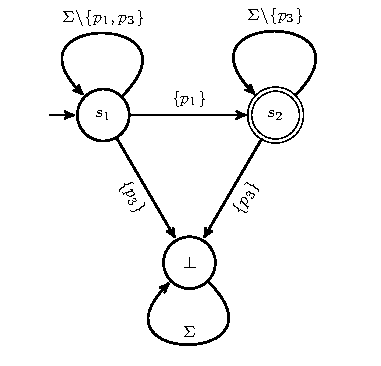
\includegraphics[width=\textwidth]{images/example_1_graph}
%		\caption{$\bot\Release(\neg p_3\vee p_1\vee p_2) \wedge \top\mathcal{U}p_1$}
%		\label{fig:g1}
%	\end{subfigure}
%	\hfill
%	\begin{subfigure}[b]{0.45\textwidth}
%
%	\end{subfigure}
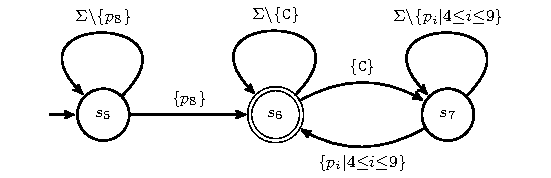
\includegraphics[scale=0.9]{images/example_3_graph}
%\caption{$\bot\Release(\neg\texttt{A}\vee(\top\Until(p_2\vee p_3)))\wedge\top\Until p_3$}
%\label{fig:g2}
	\caption{Representation of the LTL$_f$ formula $\lglobally(\neg\texttt{C}\vee(\lfuture(p_4\vee p_5\vee p_6\vee p_7\vee p_8\vee p_9)))\wedge \lfuture p_8$  as a constraint automaton \cite{Westergaard11}, where $\Sigma$ contains all the non-$\bot$ and non-$\top$ atoms.}
	\label{fig:g1g2}
\end{figure}

\section{Working Assumptions}\label{sec:wa}

In this section, we outline some working assumptions that can be inferred from the literature of reference. First, we assume that \begin{enumerate*}[label=\emph{\alph*})]
\item compliance requirements of Declare models can be expressed in a formal language such as Linear Time Logic on Finite Traces (LTL$_f$) \cite{10.1007/978-3-642-40176-3_8}, as business process logs contain only traces of finite length \cite{GiacomoV13};
\item we restrict the space of the possible alignments of the log trace repairs to the traces generated by the automaton representation of the Declare model;
%\item as in \cite{XuLZ17a}, we want to align a single log trace against a declare model, thus restricting the space of the possible alignments;
\item differently from \cite{MultiPerspective}, we can avoid to model reading and writing operation, as the entirety of our analysis will be conducted \textit{post-mortem}; \item last, each event trace must be represented by one single proposition: similarly to the non-data aware scenario \cite{XuLZ17a}, each event trace should be associated to just one activity label. \end{enumerate*} As we will see in the incoming section, the latter consideration will require us to partition the possible data space into distinct propositions.


%Still, we can freely assume that the constraint automatons generated from the LTL$_f$ interpretation of such Declare constraints allow to represent any possible event label that is not represented within the Declare constraints, by either representing it as a transition $\Sigma\backslash S$, where $\Sigma$ is the set of all the possible strings and $S$ is a (possibly empty) finite set of traces that we want to ignore \cite{LeoniMA12,Westergaard11}, or by representing it as finite conjunction of negated predicates \cite{Lydia}, where each predicate is a proposition that can be deduced from a Declare Model represented in LTL$_f$. Figure~\ref{fig:g1g2} provides a intuitive representation of some LTL$_f$ formulae in the former representation.


Given an appropriately chosen set $\Sigma$ of atoms, it is always possible to represent a trace $\sigma=\sigma_1\cdots \sigma_n$ as a finite sequence $t_\sigma=t_1\cdots t_n$, where, for $1\leq i\leq n$, $t_i$ is a unique atom $t_i\in\Sigma$ such that $\sigma_i\vDash t_i$ \cite{XuLZ17a}.
Contextually,  any LTL$_f$ formula $\varphi_{\mathcal{M}}$ representing a Declare model $\mathcal{M}$ can be represented as a deterministic finite-state automaton (DFA) $\mathcal{A}_{\varphi_{\tiny\mathcal{M}}}$ \cite{Westergaard11} accepting all the sequences $t_\sigma$ from traces $\sigma$ satisfying $\varphi_{\mathcal{M}}$ (see Figure~\ref{fig:g1g2}). A DFA  $(\Sigma,Q,q_0,\rho,F)$ is defined \cite{0016921} over a finite set of states $Q$ reading as input symbols from a finite alphabet $\Sigma$ that are consumed by traversing the automaton from a starting state $q_0\in Q$ via a transition function $\rho\colon Q\times \Sigma\to Q$; the input sequence is accepted once the input sequence is completely digested and an accepting state in $F\subseteq Q$ is reached through navigation. Given that in the non data-aware Declare scenario the atoms within LTL$_f$ could be either $\top$, or $\bot$, or $\psi=\texttt{A}$, $\Sigma$ corresponds to the activity set  $\textsf{Act}$, as each event is associated to one single label. For data-aware Declare we will extend $\Sigma$ to take into consideration propositional formulas representing data conditions.

Last, we freely assume that all the events having the same label will always contain the same set of keys, with possibly differently associated values. This is a common assumption in the relational database field, where all the rows belonging to the same table contain the same number of values. We also freely assume that missing values are represented with specific values, such as an empty string, $-1$, $0$, $-\infty$, or $+\infty$, depending on the context. 